\documentclass[a4paper, 12pt]{article}

\usepackage{hyperref}
\usepackage[warn]{mathtext}
\usepackage[utf8]{inputenc}
\usepackage[T2A]{fontenc}
\usepackage[english,russian]{babel}
\usepackage{multirow}
\usepackage{amsmath,amsfonts,amssymb,amsthm,mathtools}
\usepackage{indentfirst}
\DeclareSymbolFont{T2Aletters}{T2A}{cmr}{m}{it}
\usepackage{ gensymb }
\mathtoolsset{showonlyrefs=true}
\usepackage{euscript}
\usepackage{mathrsfs}
\usepackage[left=2cm,right=2cm,top=2cm,bottom=2cm]{geometry}
\usepackage{graphicx}
\usepackage{wrapfig}
\usepackage[rgb]{xcolor}
\hypersetup{
colorlinks=true,
urlcolor=blue
}


\title{Лабораторная работа}
\author{Гисич Арсений Б03-109}
\date{2022}

\begin{document}

	\begin{center}
		{\large МОСКОВСКИЙ ФИЗИКО-ТЕХНИЧЕСКИЙ ИНСТИТУТ (НАЦИОНАЛЬНЫЙ ИССЛЕДОВАТЕЛЬСКИЙ УНИВЕРСИТЕТ)}
	\end{center}
	\vspace{5 cm}
	{\Large
		\begin{center}
			{\bf Лабораторная работа 2.1.1}\\[0.2 cm]
			Измерение удельной теплоёмкости воздуха при постоянном давлении
		\end{center}
	}
	\vspace{4 cm}
	\begin{flushright}
		{\Large Выполнил: \\
			\vspace{0.2 cm}
			Гисич Арсений \\
			\vspace{0.2 cm}
			Б03-109 \\}
	\end{flushright}
	\vspace{8 cm}
	\begin{center}
		Долгопрудный\\[0.1 cm]
		2022
	\end{center}
\thispagestyle{empty}

\section{Аннотация}

\par Цель работы: измерить повышение температуры воздуха в зависимости от мощности
подводимого тепла и расхода при стационарном течении через трубу; исключив тепловые потери, по результатам измерений определить теплоёмкость воздуха при постоянном давлении.

\section{Теоретические сведения}

Измерение теплоёмкости тел обычно производится в калориметрах, т.е. в сосудах, обеспечивающих теплоизоляцию исследуемого тела от внешней среды. При этом регистрируется изменение его температуры $\delta T$ в зависимости от количества тепла $\delta Q$, полученного телом от некоторого нагревательного элемента внутри калориметра. Теплоёмкость тела в некотором процессе определяется как их отношение:
\begin{equation}\label{1}
C = \dfrac{\delta Q}{\delta T}.
\end{equation}

Надёжность измерения определяется, в основном, качеством калориметра. Необходимо, чтобы количество тепла, затрачиваемое на нагревание исследуемого тела, существенно превосходило тепло, расходуемое на нагревание самого калориметра, а также на потери тепла из установки. При измерении теплоёмкости газов эти требования выполнить довольно трудно - масса газа в калориметре и, следовательно, количество тепла, идущее на его нагревание, как правило, малы. Для увеличения количества нагреваемого газа при неизменных размерах установки в нашей работе исследуемый газ (воздух) продувается через калориметр, внутри которого установлен нагреватель. При этом измеряются мощность нагревателя, масса воздуха, протекающего в единицу времени (расход), и приращение его температуры.

\begin{wrapfigure}{r}{0.6\textwidth}
  \begin{center}
    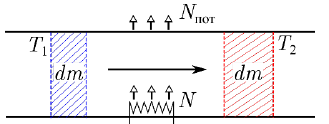
\includegraphics[width = 0.6\textwidth]{1.png}
  \end{center}
  \caption{Нагрев газа при течении по трубе}
  \label{ris1}
\end{wrapfigure}

Рассмотрим газ, протекающий стационарно слева направо через трубу постоянного сечения, в кото-рой установлен нагревательный элемент (см.рис.1). Пусть за некоторое время $dt$ через калориметр прошла малая порция газа массой $dm = q dt$ , где $q$ [кг/с] - массовый расход газа в трубе. Если мощность нагрева равна $N$, мощность тепловых потерь на обмен с окружающей средой $N_{\text{пот}}$, то порция получила тепло $\delta Q =(N - N_{\text{пот}})dt$. С другой стороны, по определению теплоёмкости
\eqref{1}: $\delta Q =c dm \Delta T$ , где $\Delta T = T_2 - T_1$ - приращение температуры газа, и $c$ — удельная (на единицу массы) теплоёмкость газа в рассматриваемом процессе. При малых расходах газа и достаточно большом диаметре трубы перепад давления на её концах мал, поэтому можно принять, что $P_1 \approx P_2 = P_0$, где $P_0$ - атмосферное давление. Следовательно, в условиях опыта измеряется удельная теплоёмкость при постоянном давлении $c_P$. Таким образом, получаем
\begin{equation}\label{2}
C_p = \dfrac{N - N_{\text{пот}}}{q \Delta T}.
\end{equation}

\section{Методика измерений}

Схема установки изображена на рис. \ref{ris2}. Воздух, нагнетаемый компрессором, прокачивается через калориметр. Калориметр представляет собой стеклянную цилиндрическую трубку с двойными стенками, запаянными с торцов. На внутреннюю поверхность стенок трубки нанесено серебряное покрытие для минимизации потерь тепла за счет излучения. Воздух из пространства между стенками калориметра откачан до высокого вакуума ($10^{-5}$~торр) для минимизации потерь тепла, обусловленных теплопроводностью.

\begin{figure}[h!]
\begin{center}
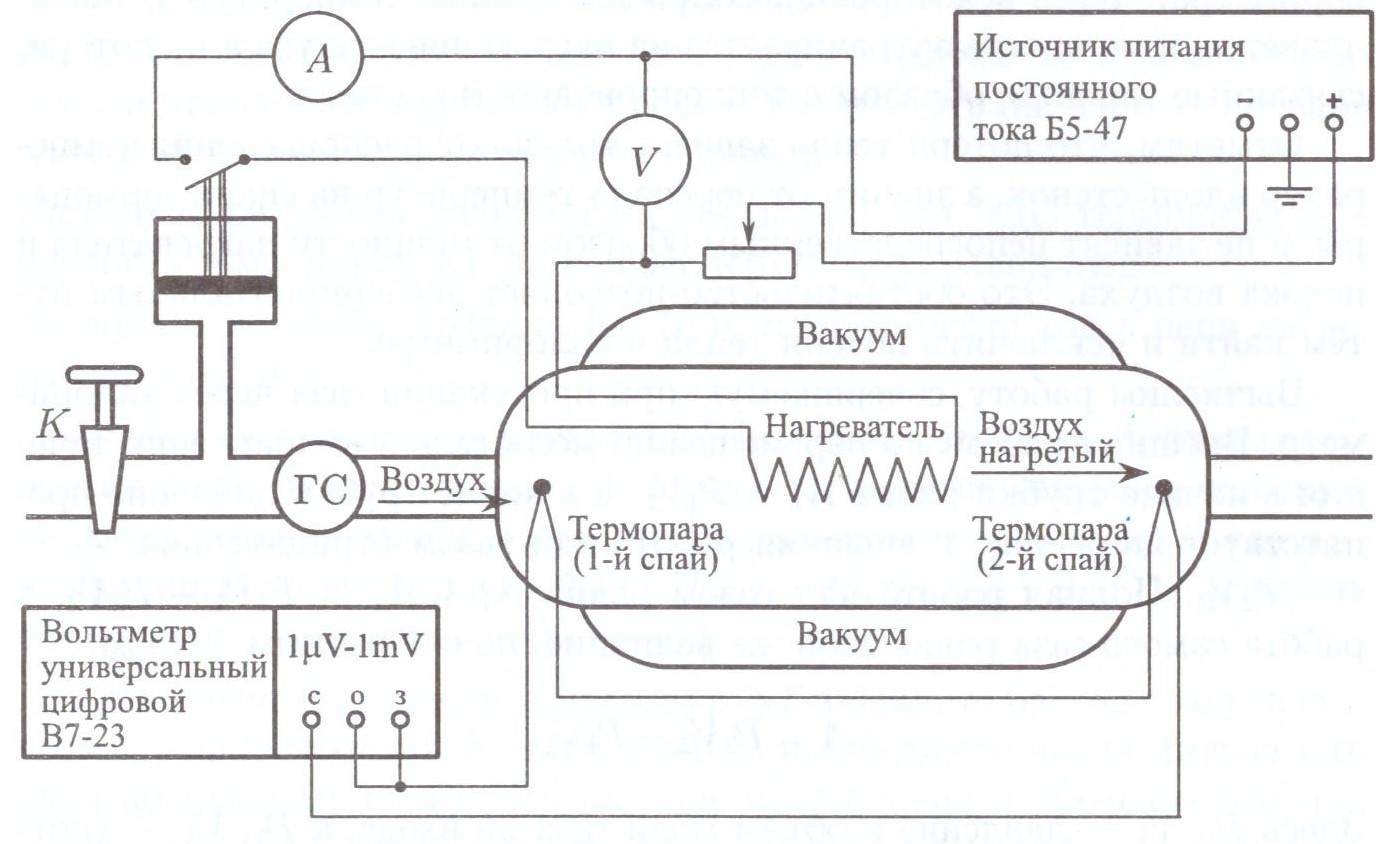
\includegraphics[width = 0.8\textwidth]{2.jpg}
\caption{Схема экспериментальной установки}
\label{ris2}
\end{center}
\end{figure}

Нагреватель в виде намотанной на пенопласт нихромовой проволоки раcположен внутри калориметра непосредственно в воздушном потоке. Нагрев проволоки производится от регулируемого источника постоянного тока (ИП). Напряжение $U$ на нагревателе и ток $I$ через него регистрируются цифровыми мультиметрами. Таким образом, мощность нагрева равна
\begin{equation}\label{3}
N = UI.
\end{equation}

Для измерения разности температур $\Delta T$ служит медно-константановая термопара. Один спай термопары расположен в струе воздуха, входящего в калориметр, и находится при комнатной температуре, а второй - в струе выходящего нагретого воздуха. Константановая проволока термопары расположена внутри калориметра, а медные проводники подключены к цифровому вольтметру. Возникающая в термопаре ЭДС $\varepsilon$ пропорциональна разности температур $\Delta T$ спаев:
\begin{equation}\label{4}
\varepsilon = \beta \Delta T,
\end{equation}
где $\beta = 40,7~\dfrac{\text{мкВ}}{ ^{\circ} C}$ -- чувствительность медно-константановой термопары в рабочем диапазоне температур (20-30 $ ^{\circ} C$). ЭДС регистрируется с помощью микровольтметра.

Объём воздуха, прошедшего через калориметр, измеряется газовым счётчиком ГС. Для регулировки расхода служит кран К. Время $\Delta t$ прохождения некоторого объема $\Delta V$ воздуха измеряется секундомером. Объёмный расход равен $\Delta V / \Delta t$, массовый расход может быть найден как
\begin{equation}\label{5}
q = \rho_0 \dfrac{\Delta V}{\Delta t},
\end{equation}
где $\rho_0$ -- плотность воздуха при комнатной температуре, которая в свою очередь может быть получена из уравнения Менделеева–Клапейрона: $\rho_0 = \dfrac{\mu P_0}{RT_0}$, где $P_0$ -- атмосферное давление, $T_0$ -- комнатная температура (в Кельвинах), $\mu$ = 29,0 г/моль -- средняя молярная масса (сухого) воздуха.

Учитывая особенности устройства калориметра, следует ожидать, что мощность нагревателя расходуется не только на нагрев массы прокачиваемого воздуха, но и частично теряется за счет нагрева внутренних стенок термостата и рассеяния тепла через торцы термостата. Можно предположить, что при небольшом нагреве ($\Delta T << T_0$) мощность потерь тепла $N_{\text{пот}}$ прямо пропорциональна разности температур:
\begin{equation}\label{6}
N_{\text{пот}} = \alpha \Delta T,
\end{equation}
где $\alpha$ — некоторая константа. При этом условии основное соотношение \eqref{2} принимает вид
\begin{equation}\label{7}
N = (c_p q + \alpha) \Delta T.
\end{equation}

Следовательно, при фиксированном расходе воздуха ($q = const$) подводимая мощность и разность температур связаны прямой пропорциональностью ($\Delta T (N)$ — линейная функция).

\section{Используемое оборудование}

\begin{enumerate}
    \item теплоизолированная стеклянная трубка;
    \item электронагреватель;
    \item источник питания постоянного тока;
    \item амперметр, вольтметр (цифровые мультиметры), $\delta_{А} = 0,1~мА;\quad \delta_{В} = 1~мВ$;
    \item термопара, подключенная к микровольтметру;
    \item компрессор;
    \item газовый счётчик, $\delta_{сч} = 0,01~л$;
    \item секундомер, $\delta_{сек} = 0,2~c$.
\end{enumerate}

\section{Результаты измерений и обработка данных}

Начальные условия:

$\begin{aligned}
& P_{атм} = 98,14\pm0,01~кПа\\
& T = 23,7\pm0,1~\celsius
\end{aligned}$\\[0,5 cm]

Измерим максимальный расход воздуха $Q$ по формуле $$Q=\frac{\Delta{V}}{\Delta{\overline{t}}}.$$ Погрешность определяется по формуле $$\delta_{Q} = \sqrt{\left(\frac{\delta_{V}}{V}\right)^2 + \left(\frac{\delta_{\overline{t}}}{\overline{t}}\right)^2} \cdot Q.$$ Затем по формуле $$q = \frac{\mu P_{атм}}{RT} \cdot Q$$ определяем массовый расход. Полученные результаты представленны в таб. \ref{tab1}.

\begin{table}[h!]
\begin{center}
\begin{tabular}{|c|c|c|c|c|c|c|c|c|}
\hline
$t, c$ & $\overline{t}, c$     & $\delta_{\overline{t}}, c$ & $V, л$             & $\delta_V, л$         & $Q_{max}, л/c$               & $\delta_{Q_{max}}, л/c$        & $q_{max}, г/c$               & $\delta_{q_{max}}, г/c$        \\ \hline
5,08   & \multirow{5}{*}{5,14} & \multirow{5}{*}{0,46}      & \multirow{5}{*}{1} & \multirow{5}{*}{0,01} & \multirow{5}{*}{0,194} & \multirow{5}{*}{0,017} & \multirow{5}{*}{0,224} & \multirow{5}{*}{0,020} \\ \cline{1-1}
5,3    &                       &                            &                    &                       &                        &                        &                        &                        \\ \cline{1-1}
4,96   &                       &                            &                    &                       &                        &                        &                        &                        \\ \cline{1-1}
5,47   &                       &                            &                    &                       &                        &                        &                        &                        \\ \cline{1-1}
4,9    &                       &                            &                    &                       &                        &                        &                        &                        \\ \hline
\end{tabular}
\caption{Расчёт маскимального расхода}
\label{tab1}
\end{center}
\end{table}

Оценим минимальную мощность $N_0$ по формуле \eqref{7}, где $c_p = \frac{5}{2}\frac{R}{\mu}$, так как воздух считаем смесью двухатомных идеальных газов. Получаем $N_0 \approx 0,161~Вт$. Учитывая сопротивление проволоки нагревателя $R_н \sim 35~Ом$, оценим $I_0 = \sqrt{\frac{N_0}{R_н}} \approx 70 мА$.

Проведём первое измерение при $q_1 = q_{max}$. Установим начальный ток $I_1 \sim 2I_0$. Результаты измерений прдеставлены в таб. \ref{tab2}.

\begin{table}[h!]
\begin{center}
\begin{tabular}{|c|c|c|c|c|c|c|c|c|c|}
\hline
$I, мА$ & $\delta_{I}, мА$ & $U, B$ & $\delta_{U}, B$ & $N, Вт$ & $\delta_{N}, Вт$ & $\varepsilon, мкВ$ & $\delta_{\varepsilon}, мкВ$ & $\Delta{T}, \celsius$ & $\delta_{\Delta{T}}, \celsius$ \\ \hline
160,2   & 0,1              & 4,568  & 0,001           & 0,7318  & 0,0005           & 116                & 1                                                            & 2,85                  & 0,02                           \\ \hline
182     & 0,1              & 5,194  & 0,001           & 0,9453  & 0,0006           & 144                & 1                                                            & 3,54                  & 0,02                           \\ \hline
203,3   & 0,1              & 5,803  & 0,001           & 1,1797  & 0,0006           & 187                & 1                                                            & 4,59                  & 0,02                           \\ \hline
217,8   & 0,1              & 6,218  & 0,001           & 1,3543  & 0,0007           & 209                & 1                                                            & 5,14                  & 0,02                           \\ \hline
\end{tabular}
\caption{1 измерение}
\label{tab2}
\end{center}
\end{table}

Проведём второе измерение при меньшем расходе. По приведённым выше формулам найдём расход воздуха и начальный ток. Результаты измерений представленны в таб. \ref{tab3}.

\begin{table}[h!]
\begin{center}
\begin{tabular}{|c|c|c|c|c|c|c|c|c|}
\hline
$t, c$ & $\overline{t}, c$     & $\delta_{\overline{t}}, c$ & $V, л$             & $\delta_V, л$         & $Q_{max}, л/c$               & $\delta_{Q_{max}}, л/c$        & $q_{max}, г/c$               & $\delta_{q_{max}}, г/c$ \\ \hline
14,09 & \multirow{5}{*}{13,76} & \multirow{5}{*}{0,48} & \multirow{5}{*}{1} & \multirow{5}{*}{0,01} & \multirow{5}{*}{0,073} & \multirow{5}{*}{0,003} & \multirow{5}{*}{0,084} & \multirow{5}{*}{0,003} \\ \cline{1-1}
13,85 &                        &                       &                    &                       &                        &                        &                        &                        \\ \cline{1-1}
13,21 &                        &                       &                    &                       &                        &                        &                        &                        \\ \cline{1-1}
14,1  &                        &                       &                    &                       &                        &                        &                        &                        \\ \cline{1-1}
13,55 &                        &                       &                    &                       &                        &                        &                        &                        \\ \hline
\end{tabular}
\end{center}
\caption{Расчёт второго расхода}
\label{tab3}
\end{table}

Минимальная мощность $N_0 = 0,057~Вт$, $I_0 = 40~мА$. Результаты измерений представленны в таб. \ref{tab4}.

\newpage
\begin{table}[h!]
\begin{center}
\begin{tabular}{|c|c|c|c|c|c|c|c|c|c|}
\hline
$I, мА$ & $\delta_{I}, мА$ & $U, B$ & $\delta_{U}, B$ & $N, Вт$ & $\delta_{N}, Вт$ & $\varepsilon, мкВ$ & $\delta_{\varepsilon}, мкВ$ & $\Delta{T}, \celsius$ & $\delta_{\Delta{T}}, \celsius$ \\ \hline
96,3  & 0,1 & 2,742 & 0,001 & 0,2641 & 0,0003 & 86  & 1 & 2,11 & 0,02 \\ \hline
127,6 & 0,1 & 3,638 & 0,001 & 0,4642 & 0,0004 & 151 & 1 & 3,71 & 0,02 \\ \hline
180,1 & 0,1 & 5,141 & 0,001 & 0,9259 & 0,0005 & 262 & 1 & 6,44 & 0,02 \\ \hline
214,7 & 0,1 & 6,135 & 0,001 & 1,3172 & 0,0006 & 383 & 1 & 9,41 & 0,02 \\ \hline
\end{tabular}
\caption{2 измерение}
\label{tab4}
\end{center}
\end{table}

График зависимости $\Delta{T}(N)$ представлен на рис. \ref{ris3}.
\begin{figure}[h!]
\begin{flushleft}
    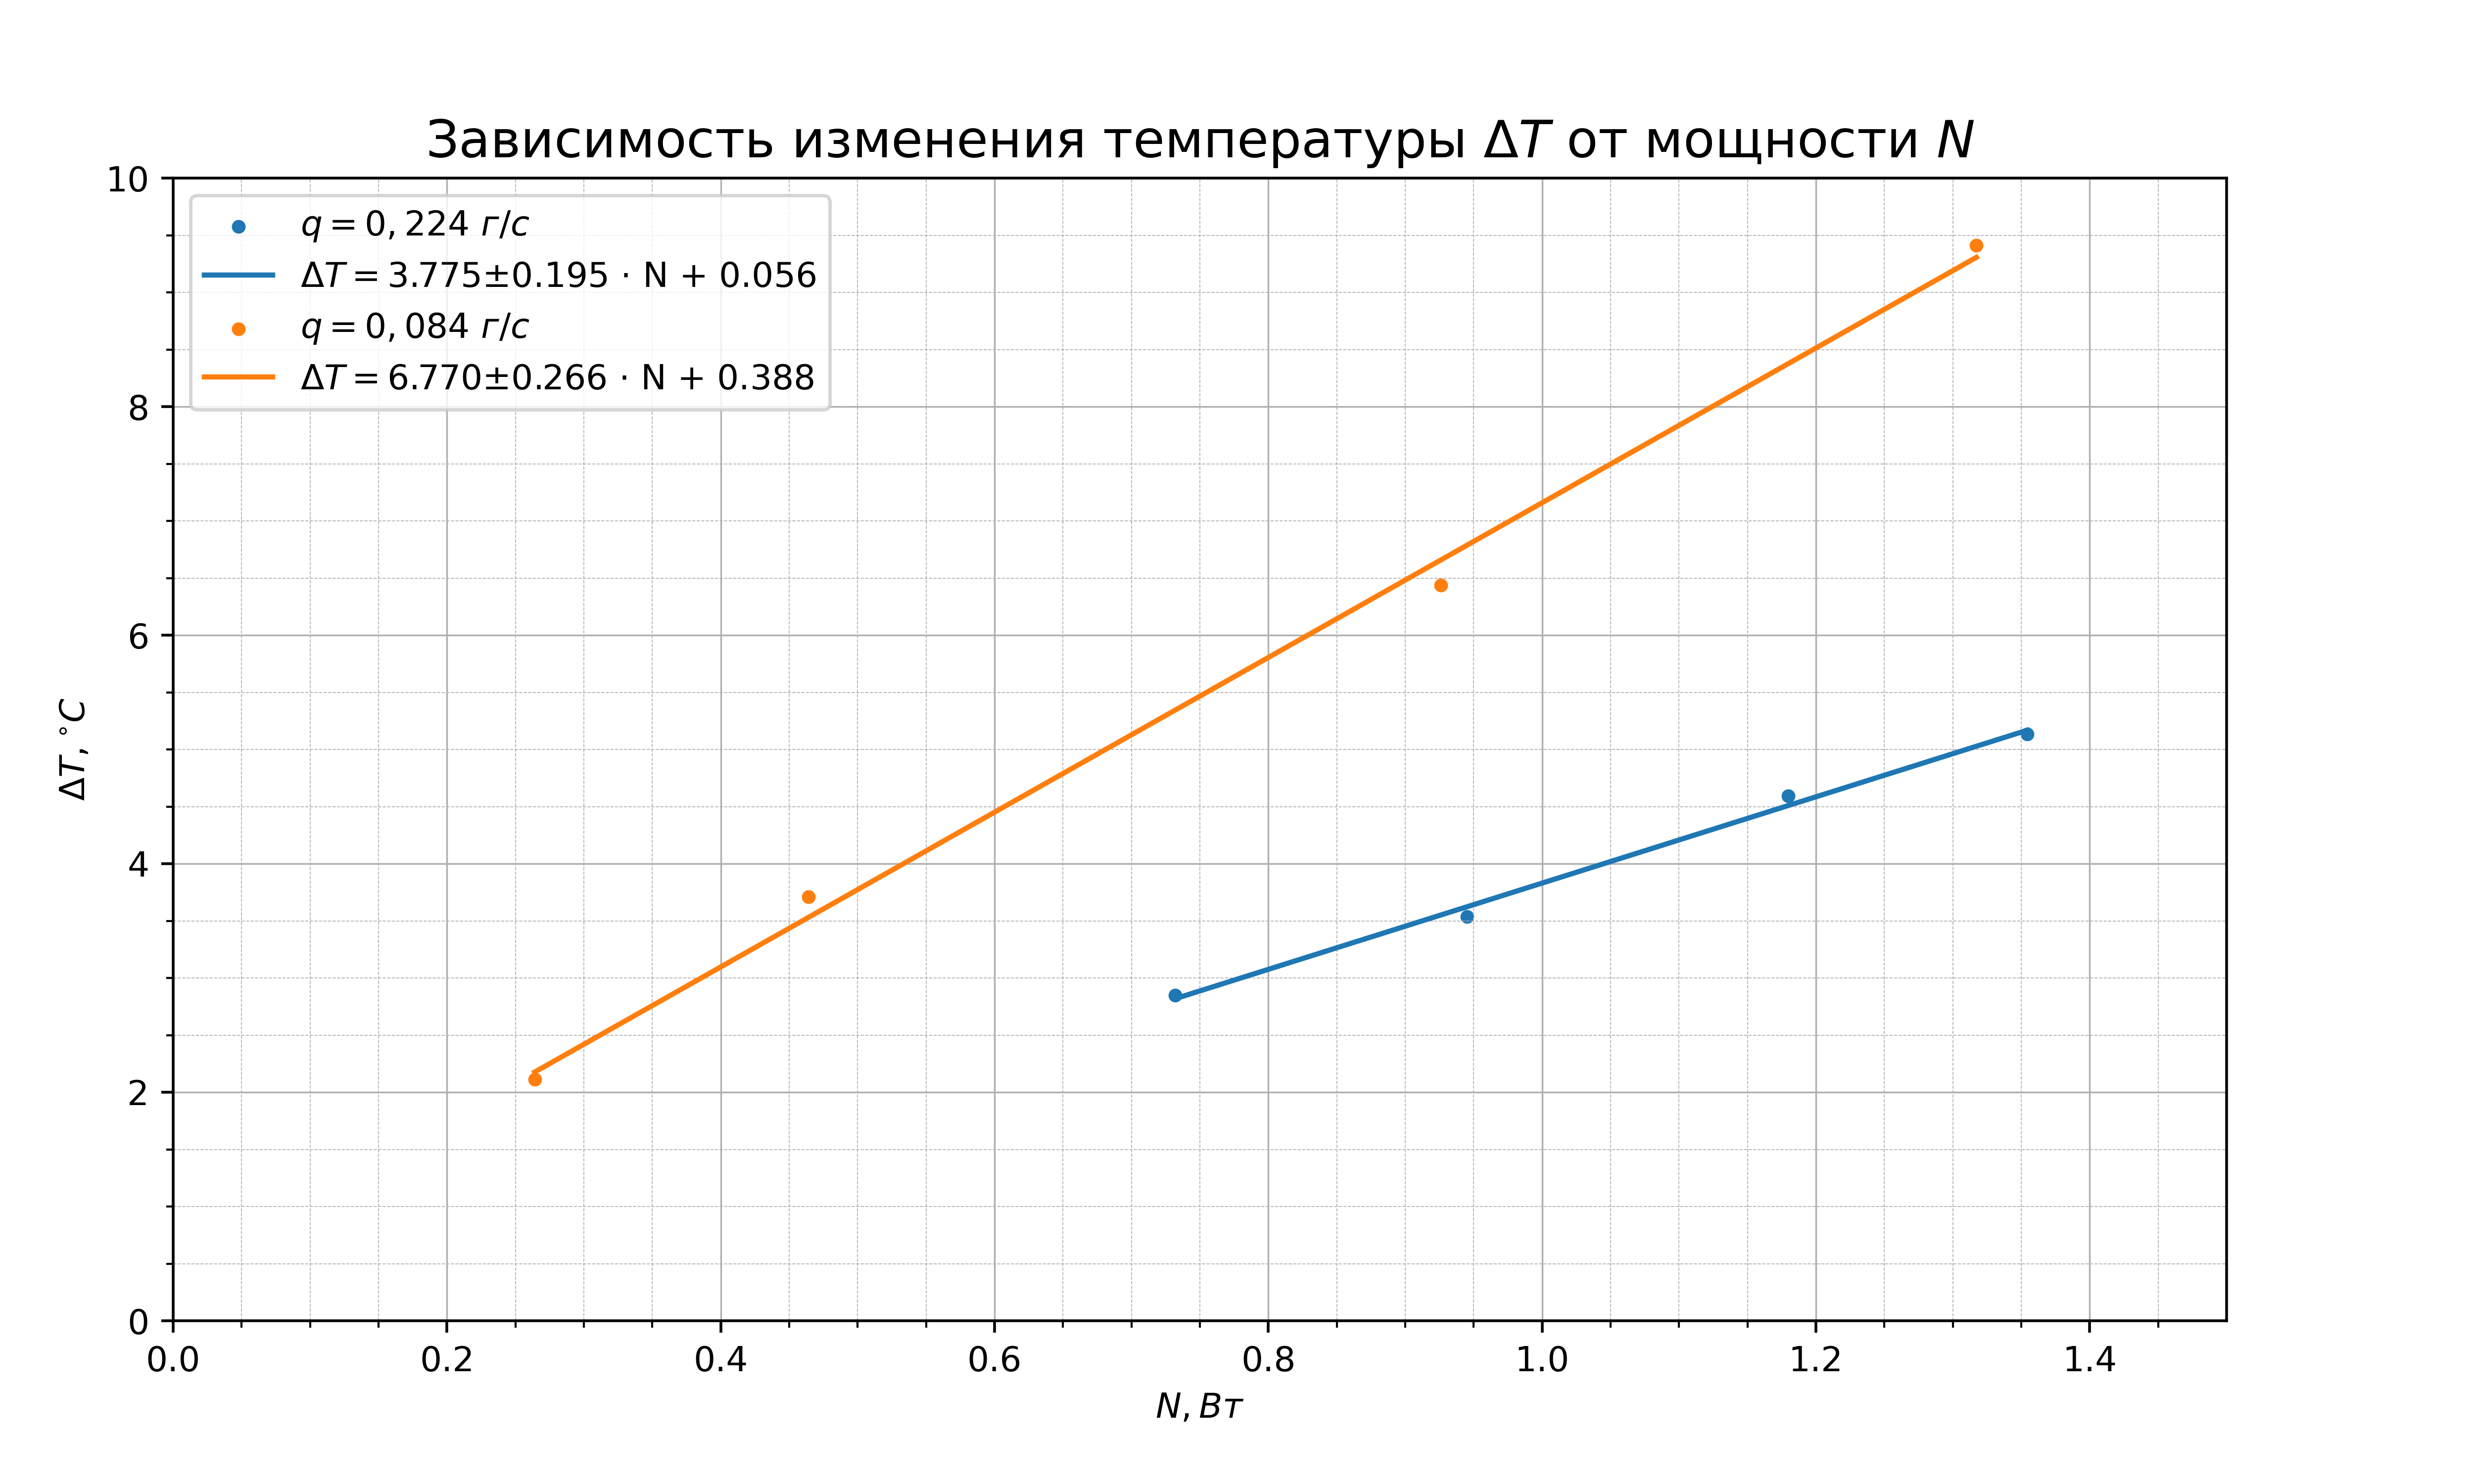
\includegraphics[scale=0.75]{2.1.1.png}
\end{flushleft}
\caption{}
\label{ris3}
\end{figure}

Из формулы \eqref{7} получаем $$c_p = \left(\frac{1}{k_1} - \frac{1}{k_2}\right) \cdot \frac{1}{q_1 - q_2}.$$ Погрешность определяется по формуле $$\delta_{c_p} = \sqrt{\left(\frac{\left(\frac{\delta_{k_1}}{k_1^2}\right)^2 + \left(\frac{\delta_{k_2}}{k_2^2}\right)^2}{(k_1^{-1} - k_2^{-1})^2}\right) + \left(\frac{\delta_{q_1}^2 + \delta_{q_2}^2}{(q_1 - q_2)^2}\right)} \cdot c_p.$$ Получаем $$\boxed{c_p = 837,01\pm160,91~\frac{Дж}{кг \cdot K} = (2,9\pm0,6)R~\frac{Дж}{моль \cdot K}}.$$ Из формул \eqref{6} и \eqref{7} получаем $$\frac{N_{пот}}{N} = \alpha k_1 = 1 - k_1 c_p q_1.$$ Погрешность определяется по формуле $$\delta_{\frac{N_{пот}}{N}} = \sqrt{\left(\frac{\delta_{k_1}}{k_1}\right)^2 + \left(\frac{\delta_{c_p}}{c_p}\right)^2 + \left(\frac{\delta_{q_1}}{q_1}\right)^2} \cdot (1 - k_1 c_p q_1).$$ Получаем $$\boxed{\frac{N_{пот}}{N} = 0,29\pm0,06}.$$

\section{Обсуждение результатов и выводы}

В данной работе исследовалась зависимость давления в установке от времени. По результатам измерения давления различными способами определялась производительность вакуумного насоса. Полученное значение для скорости откачки:
\[\boxed{W = 0,258\pm0,012~л/с}.\]
Использованный в работе метод измерений позволяет достичь относительной точности результатов в 5\%. Метод расчёта скорости откачки по зависимости давления от времени при улучшении вакуума оказался точнее в сравнении с методом расчёта по различию $P_{уст}$ и $P_{пр}$. Основной вклад в погрешность вносит погрешность определения коэффициентов линейной аппроксимации.
Также в данной работе были проверены теоретические зависимости, связанные с течением газа ().

\end{document}
